\documentclass{beamer}
\usepackage[utf8]{inputenc}
\usepackage[portuguese]{babel}
\usepackage{amsthm}
\usepackage{amssymb, bm}
\usepackage{ragged2e}
\usepackage{graphicx}
\usepackage{pythonhighlight}


%%% Tema Customizado para o Beamer
\usefonttheme{serif}

\setbeamertemplate{footline}[frame number]{}
\setbeamertemplate{navigation symbols}{}

\usecolortheme{lily}
\setbeamercolor{block title}{bg=blue!20,fg=black}
\setbeamercolor{block body}{bg = blue!10, fg = black}
\setbeamertemplate{itemize item}[square]
\setbeamercolor{itemize item}{fg = blue}
\setbeamercolor{enumerate item}{fg = blue}

\usetheme{default}
\beamertemplatenavigationsymbolsempty
\setbeamercolor{titlelike}{fg=blue}
%%%

\graphicspath{{./imagens/}}

\theoremstyle{definition}
\newtheorem{qst}{Teorema}

\title{Regressão: \textit{Naval Propulsion Plants}}
\author{Carolina Dias}
\date{Maio de 2022}

\begin{document}

\maketitle

\begin{frame}{Conteúdo}
\begin{enumerate}
    \item Aplicações da Regressão Linear
    \item Regressão Linear: Método dos Mínimos Quadrados
    \item Conjunto de Dados: Indústria Naval
    \item Experimentos
    \item Resultados
\end{enumerate}
\end{frame}


\begin{frame}{Aplicações da Regressão Linear}
\justifying
\begin{itemize}
    \item Legendre em 1805 e Gauss em 1809: primeira aplicação na \textbf{predição de movimentos planetários}.
    \pause
    \item Prever \textbf{quantidade de itens vendidos de um produto} com informações sobre quantidade de pessoas na loja.
    \pause
    \item Encontrar a \textbf{dosagem de um medicamento deve ser aplicada em um paciente} com informações sobre seu peso e outros dados fisiológicos.
    \pause
    \item Análise da \textbf{qualidade de alimentos}, utilizando dados como a qualidade da água utilizada.
    \pause
    \item Aproximação de \textbf{dados sobre a poluição do ar pela concentração de NO em uma cidade}, com informações sobre a quantidade de carros em cada período durante um dia.
\end{itemize}
    
\end{frame}


\begin{frame}{Regressão Linear: Método dos Mínimos Quadrados}
\justifying
O \textbf{Método dos Mínimos Quadrados} consiste em encontrar uma solução aproximada, $\mathbf{\tilde{x}}$, de um sistema inconsistente

$$A\mathbf{x} = \mathbf{b}.$$

Isso é feito projetando o vetor $\mathbf{b}$ no espaço-nulo esquerdo de $A$ e resolvendo as equações normais

$$A^TA\mathbf{\tilde{x}} = A^T\mathbf{b}.$$

Pode-se substituir $A$ por sua decomposição QR, $A = QR$, e obter novas equações normais:

$$R\mathbf{\tilde{x}} = Q^T\mathbf{b},$$

sob determinadas condições em $A$.
    
\end{frame}

\begin{frame}{Conjunto de Dados: Indústria Naval}
\justifying
Utilizamos um conjunto de dados relacionado à Fábrica de Propulsões Navais (\textit{Naval Propulsion Plants}). Esses dados foram gerados através de um simulador numérico de turbinas de gás.

\begin{itemize}
    \item \textbf{11.934 medições},
    \item \textbf{16 atributos},
    \item \textbf{2 variáveis dependentes},
    \item Total: \textbf{vetor com 18 valores}.
\end{itemize}
\pause
    
 Tratamos das variáveis dependentes uma por vez, separadamente. Inicialmente, utilizamos a \textit{GT Compressor decay state coefficient} (chamamos de \textbf{GTC}). Para a outra variável dependente, a \textit{GT Turbine decay state coefficient} (\textbf{GTT}), o processo é análogo.
   
\end{frame}

\begin{frame}{Conjunto de Dados: Indústria Naval}
\justifying
Queremos encontrar solução para o \textbf{sistema de equações}:
    
\begin{align*}
    \alpha_1 x_{11} + \alpha_2 x_{12} + \ldots + \alpha_{16} x_{116} + \alpha_{17} &= GTC_1\\
    \alpha_1 x_{21} + \alpha_2 x_{22} + \ldots + \alpha_{16} x_{216} + \alpha_{17} &= GTC_2\\
    \vdots &= \vdots\\
    \alpha_1 x_{119341} + \alpha_2 x_{119342} + \ldots + \alpha_{16} x_{1193416} + \alpha_{17} &= GTC_{11934}
\end{align*}
\pause

Esse sistema equivale, matricialmente, à

$$
\begin{bmatrix}
    x_{11} & x_{12} & \dots & x_{116} \\
    x_{21} & x_{22} & \dots & x_{216} \\
    \vdots & \vdots & \ddots & \vdots \\
    x_{119341} & x_{119342} & \dots & x_{1193416}
\end{bmatrix}
\begin{bmatrix}
    \alpha_1 \\
    \alpha_2 \\
    \vdots\\
    \alpha_{16}
\end{bmatrix}
=
\begin{bmatrix}
    GTC_1 \\
    GTC_2 \\
    \vdots\\
    GTC_{11934}
\end{bmatrix}
$$
   
\end{frame}


\begin{frame}{Experimentos}
\justifying
\textbf{Requisitos:} \textit{Python} 3.8.10 e \textit{Jupyter Notebook}.

\begin{itemize}
    \item \textbf{Download e leitura do conjunto de dados}, utilizando a biblioteca \textit{Pandas}.
    \item Criação de funções auxiliares.
\end{itemize}
\pause

Queremos que nosso conjunto de dados possua \textbf{n colunas linearmente independentes}, onde \textbf{n = posto(A)}. Vamos \textbf{calcular o posto da matriz de dados original após a remoção das duas variáveis independentes}, ou seja,\textbf{ 16 variáveis restantes}. \textbf{Adicionamos uma coluna composta apenas do número 1 ao final da matriz}. Ficamos com um \textbf{vetor de tamanho 17}. Ao calcularmos o posto dessa matriz, utilizando a função do \textit{NumPy} \textit{linalg.matrix\_rank()}, obtemos que $\mathbf{posto(A) = 14}$. Ou seja, \textbf{existem 3 colunas que são linearmente dependentes} nesse conjunto de dados.

\end{frame}

\begin{frame}{Experimentos}
\justifying
Para encontramos essas colunas, podemos realizar a \textbf{decomposição LU} da matriz A, $A = LU$ e encontrar as colunas correspondentes às colunas sem pivôs na matriz $U$. Mas, nesse caso, isso não é necessário. Ao olharmos para a matriz A, conseguimos observar que \textbf{existem duas colunas constantes e uma coluna que é repetição de outra}. Confirmamos que esse é realmente o caso, com funções específicas do \textit{NumPy} e do \textit{Pandas}, e removemos essas colunas do conjunto de dados.
\newline\\
\pause

Agora possuímos um conjunto de dados em forma de matriz com \textbf{14 variáveis} e, ao conferir o posto dessa matriz, vemos que ele é 14. Isso nos diz que agora \textbf{todas as colunas são linearmente independentes}, e podemos prosseguir para o cálculo da decomposição QR de A, do modo detalhado acima.

\end{frame}

\begin{frame}{Experimentos}
\justifying
\begin{itemize}
    \item Com a matriz com todas as colunas linearmente independentes, a \textbf{separamos em dados de treino e teste}. Ficamos, assim, com 4 matrizes: \textit{X\_train, y\_train, X\_test, y\_test}.
    \pause
    \item Finalmente, \textbf{calculamos a decomposição QR da matriz de treinamento} \textit{X\_train}, já com a coluna de 1s $[1\ 1\ \ldots\ 1]^T$ adicionada.
    \pause
    \item Agora \textbf{encontramos os coeficientes lineares} $[\alpha_1, \alpha_2, \ldots, \alpha_{14}]$ com o comando\\ \pyth{coefs_lineares = np.linalg.solve(R, np.dot(Q.T, y_train))}
\end{itemize}

\end{frame}

\begin{frame}{Experimentos}
\justifying
\begin{itemize}
    \item Com os coeficientes lineares podemos \textbf{calcular os valores de $GTC$}, a primeira variável dependente, para cada um dos vetores medidos, tanto para o conjunto de treino, como para o conjunto de teste.
    \item Com isso podemos calcular o erro entre essa predição e o valor de fato. Utilizamos, aqui, a métrica da \textbf{raiz quadrada do erro médio quadrático} (RMSE), dada por
\pause

\begin{equation*}
\label{eqn:rmse}
RMSE = \sqrt{\frac{(y_1 - \hat{y}_1)^2 + (y_2 - \hat{y}_2)^2 + \ldots + (y_m - \hat{y}_m)^2}{m}},
\end{equation*}

sendo $m$ a dimensão dos vetores \textit{y} e \textit{y\_preds}, tanto para treino como para teste. Nesse caso, $m_{treino} = 8353$ e $m_{teste} = 3581$.
\end{itemize}

\end{frame}

\begin{frame}{Resultados}
\begin{figure}[h]
  \centering
  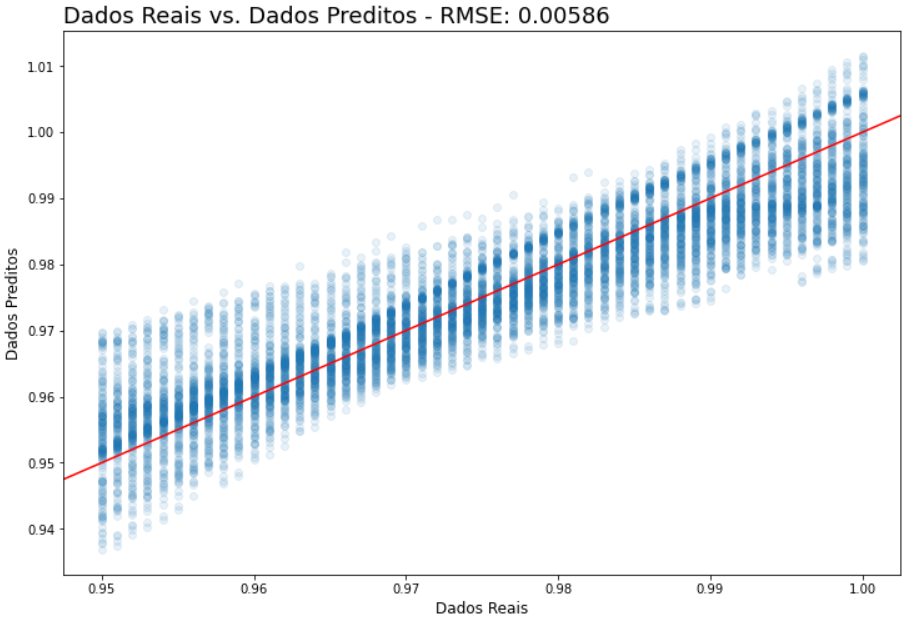
\includegraphics[width=9cm]{treinoGT}
  \caption{Resultado da predição de treino para a variável dependente $GTC$.}
  \label{fig:treinoGT}
\end{figure}
\end{frame}

\begin{frame}{Resultados}
\begin{figure}[h]
  \centering
  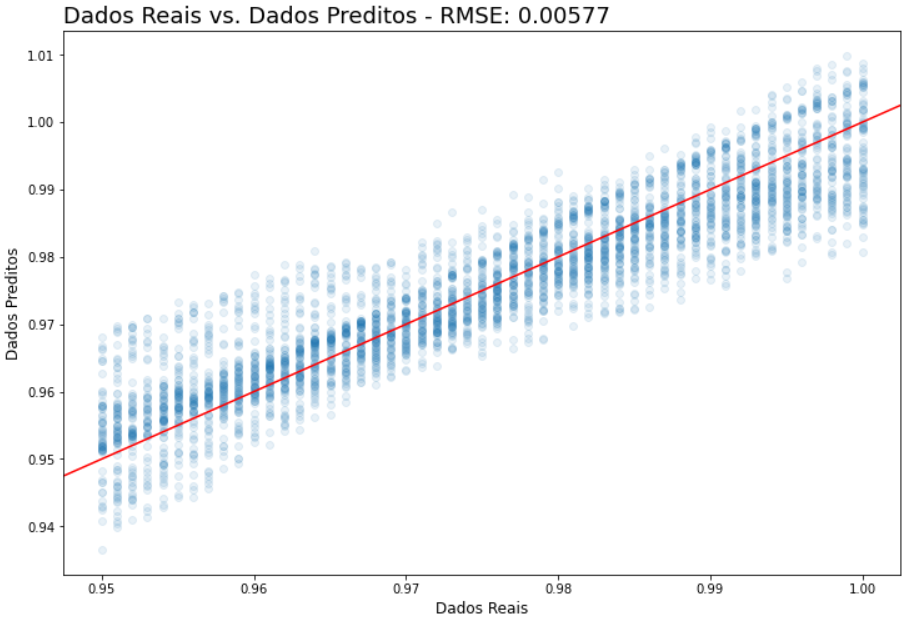
\includegraphics[width=9cm]{testeGT}
  \caption{Resultado da predição de teste para a variável dependente $GTC$.}
  \label{fig:testeGT}
\end{figure}
\end{frame}

\begin{frame}{Resultados}
\begin{figure}[h]
  \centering
  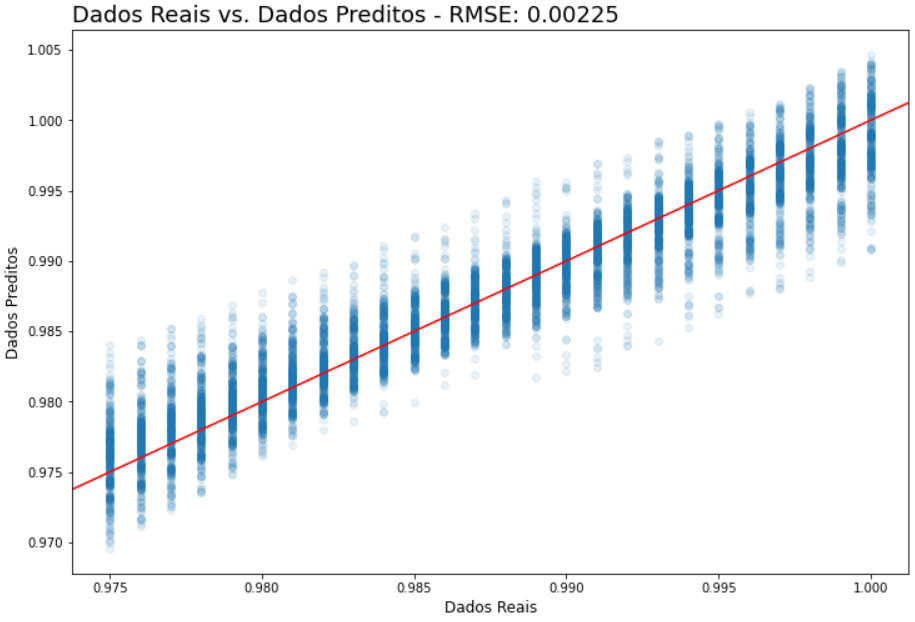
\includegraphics[width=9cm]{treinoGT1}
  \caption{Resultado da predição de treino para a variável dependente $GTT$.}
  \label{fig:treinoGT1}
\end{figure}
\end{frame}

\begin{frame}{Resultados}
\begin{figure}[h]
  \centering
  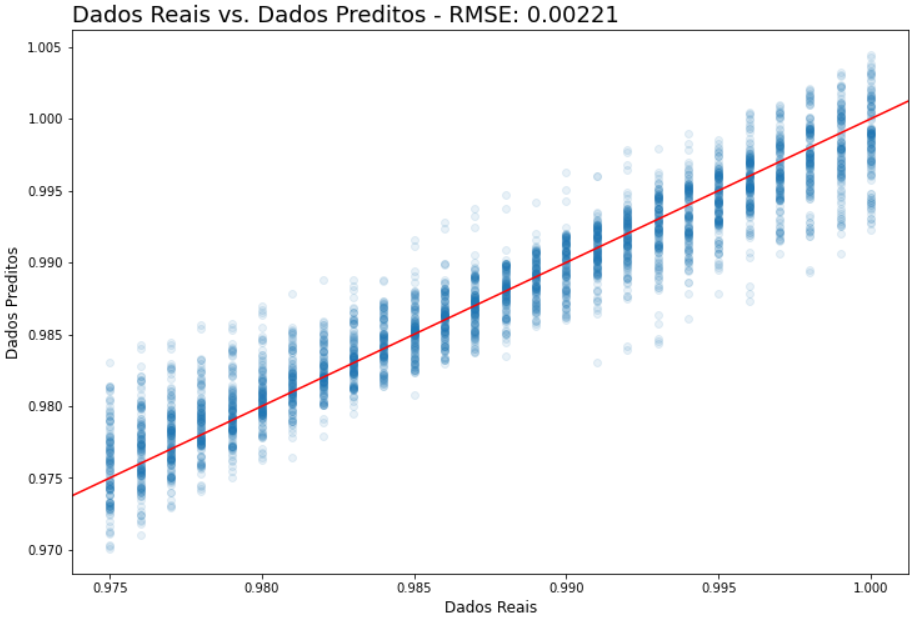
\includegraphics[width=9cm]{testeGT1}
  \caption{Resultado da predição de teste para a variável dependente $GTT$.}
  \label{fig:testeGT1}
\end{figure}
\end{frame}

\end{document}
